\documentclass[xetex]{beamer}

\usepackage{hyperref}
\usepackage{qtree}
\usepackage[no-math]{fontspec}
\usepackage{media9}

\usepackage[
  orientation=landscape,
  size=custom,
  width=16,
  height=9,
  scale=0.5
]{beamerposter}

\usefonttheme{serif}

\setmainfont[
  Path           = ./font/,
  BoldFont       = MerriweatherBold.ttf,
  ItalicFont     = MerriweatherItalic.ttf,
  BoldItalicFont = MerriweatherBoldItalic.ttf
]{MerriweatherRegular.ttf}

\definecolor{wordpressblue}{RGB}{00,135,190}

\title{wordcereal}
\subtitle{an english grammar-aware passphrase word list}
\author{nathan bloomfield}
\date{grand meetup 2017 -- whistler}


\begin{document}

\setbeamercolor{frametitle}{fg=wordpressblue}
\setbeamercolor{title}{fg=wordpressblue}



\frame{\titlepage}



\begin{frame}
\frametitle{disclosure}

prior art

\begin{itemize}
\item \url{http://copleytech.com/pass-phrases/} (powered by WP.org!)
\item \url{http://philzimmermann.com/docs/PGP_word_list.pdf}
\item \url{https://www.eff.org/deeplinks/2016/07/new-wordlists-random-passphrases}
\end{itemize}
\end{frame}



\begin{frame}
\frametitle{let's talk about passphrases}

\pause

\begin{center}
correct horse battery staple

\pause

\vspace{1cm}

memorable > short

\pause

\vspace{1cm}

grammar?
\end{center}
\end{frame}



\begin{frame}
\frametitle{let's talk about passphrases}

scary pop-press articles say grammar is bad, citing this paper:

\vspace{0.3cm}

\url{https://www.cs.cmu.edu/~agrao/paper/Effect_of_Grammar_on_Security_of_Long_Passwords.pdf}

\pause

\begin{center}
\raisebox{-0.5\height}{
\includegraphics[width=90pt]{img/the-point.png}}%
\end{center}

\end{frame}



\begin{frame}
\frametitle{let's talk about passphrases}

\begin{center}
any reversible map from bits to sentences \\ will losslessly encode entropy

\vspace{1.5cm}

\pause compromise: may need a \emph{longer} phrase
\end{center}
\end{frame}



\begin{frame}
\frametitle{how to construct an arbitrary sentence}

generative grammars (Chomsky, 1957)

\begin{center}
\raisebox{-0.5\height}{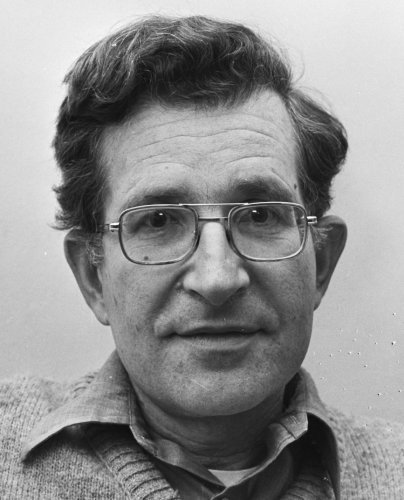
\includegraphics[width=100pt]{img/chomsky.jpg}}%
\quad\quad\quad%
\raisebox{-0.5\height}{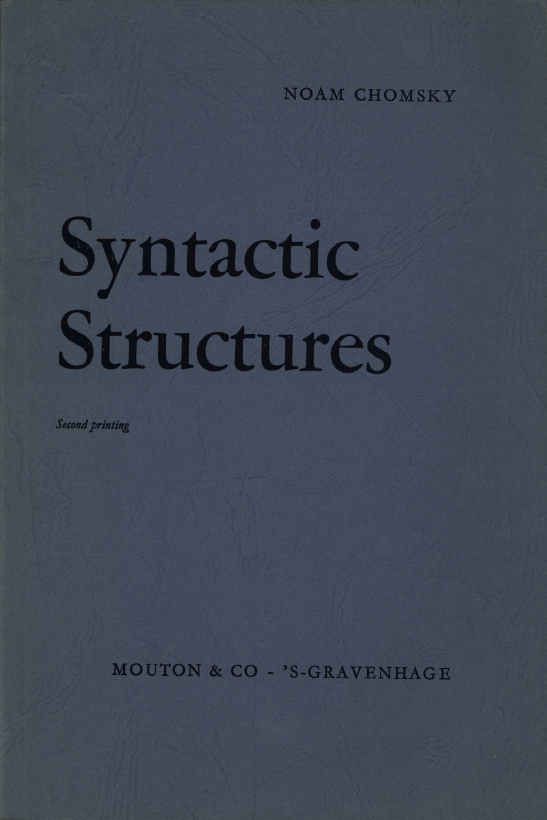
\includegraphics[width=100pt]{img/syntactic-structures.png}}%
\end{center}

\end{frame}



\begin{frame}
\frametitle{how to construct an arbitrary sentence}

mad libs (Stern and Price, 1953)

\begin{center}
\raisebox{-0.5\height}{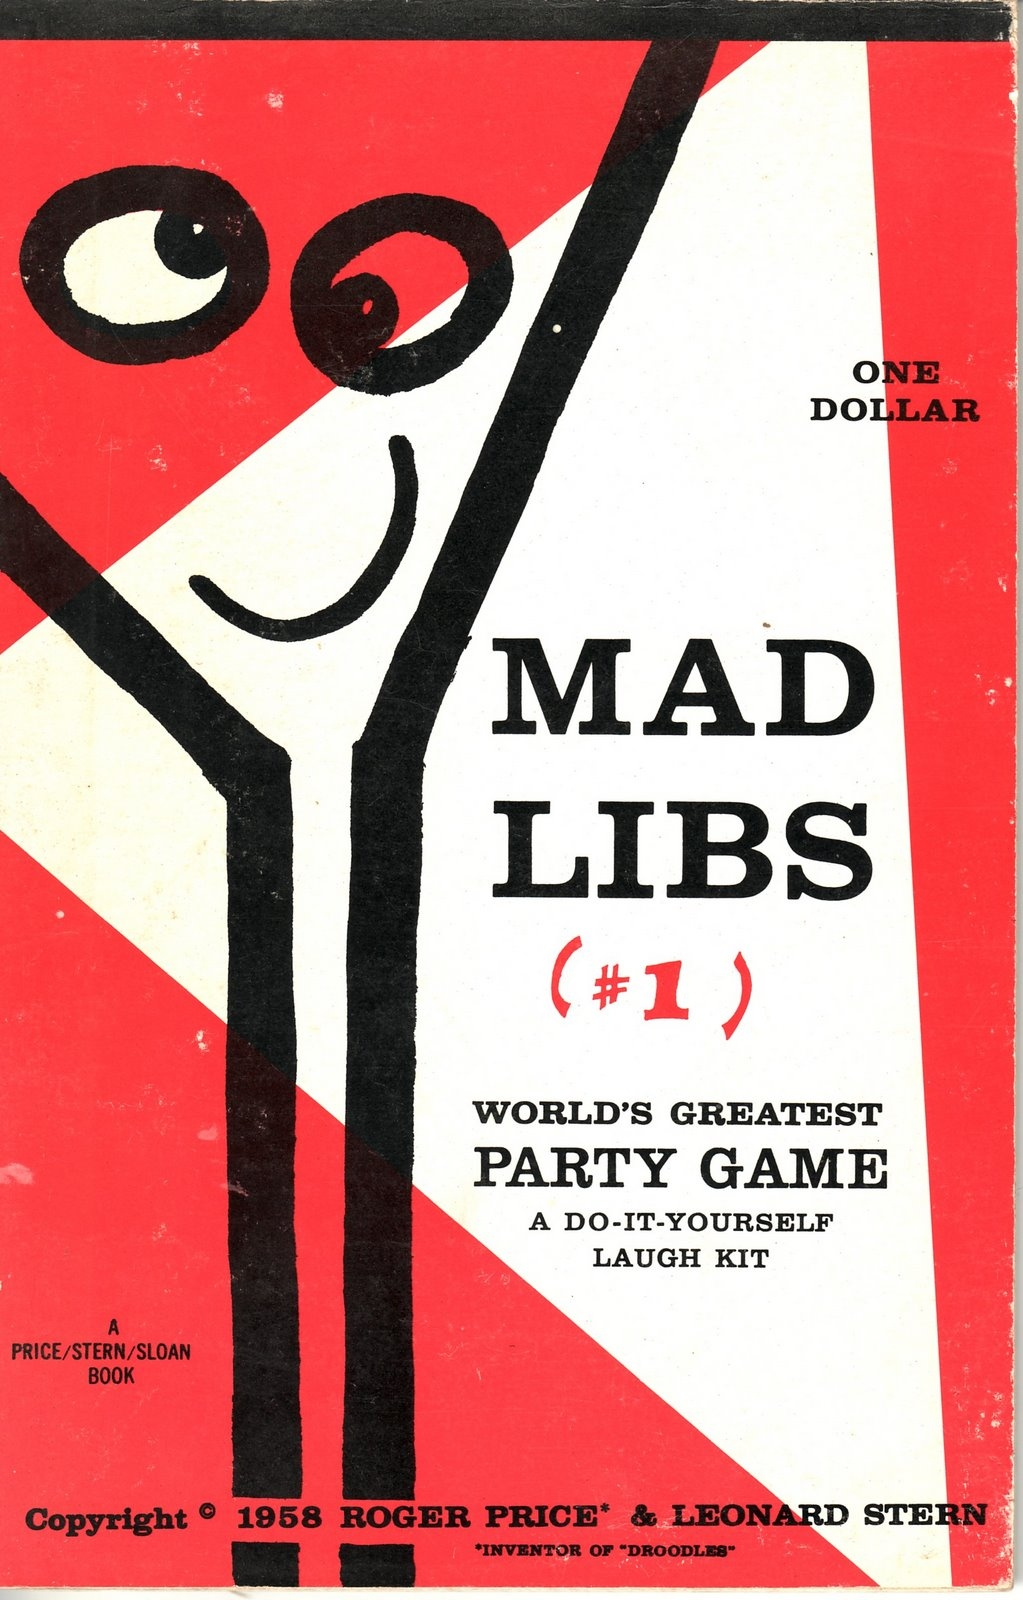
\includegraphics[height=120pt]{img/madlibs-no1.jpg}}%
\end{center}

\end{frame}



\begin{frame}
\frametitle{how to construct an arbitrary sentence}

\Tree [.S [.NP {\makebox[2cm]{colorless}} [.NP {\makebox[2cm]{green}} {\makebox[2cm]{ideas}} ] ] [.VP {\makebox[2cm]{sleep}} {\makebox[2cm]{furiously}} ] ]
\end{frame}



\begin{frame}
\frametitle{how to construct an arbitrary sentence}

\Tree [.S [.NP {\makebox[2cm]{adjective}} [.NP {\makebox[2cm]{adjective}} {\makebox[2cm]{noun}} ] ] [.VP {\makebox[2cm]{verb}} {\makebox[2cm]{adverb}} ] ]
\end{frame}



\begin{frame}
\frametitle{wordcereal}

proof of concept

\begin{center}
\url{https://github.com/nbloomf/wordcereal}
\end{center}

\pause

\begin{itemize}
\item 512 each of plural nouns, transitive verbs, adjectives, and adverbs (8 bits/word)
\item 8 each of prepositions, determiners, and conjunctions (2 bits/word)
\end{itemize}
\end{frame}



\begin{frame}
\frametitle{combinatorial properties}
\begin{itemize}
\item prefix free (and suffix free)
\item unique initial 5-grams
\item initial 3-grams decode uniquely
\item edit distance $\geq 3$
\end{itemize}
\end{frame}



\begin{frame}
\frametitle{semantic properties}
\begin{itemize}
\item avoid vulgar words
\item avoid marginalizing, ``-ist'' words
\item avoid proper nouns and trademarks
\end{itemize}
\end{frame}



\begin{frame}
\frametitle{phonetic properties}
\begin{itemize}
\item phonetically prefix free (and suffix free)
\item phonetic edit distance $\geq 1$ (this is fuzzy)
\item avoid words that are homophones
\item two lists, divided on syllable count parity (even/odd)
\end{itemize}
\end{frame}


\begin{frame}
\frametitle{examples}
\begin{center}
waterfalls deduplicate gossipy channels (32 bits)

\vspace{1cm}

those pathways vilify several schematics \\ throughout few crayons (40 bits)

\vspace{1cm}

schematics familiarize two aberrations and \\ level references lampoon lozenges (60 bits)
\end{center}
\end{frame}

\setbeamercolor{background canvas}{bg=wordpressblue}
\setbeamercolor{normal text}{fg=white}
\usebeamercolor[fg]{normal text}

\begin{frame}

\end{frame}

\end{document}
